
\subsection{Flood fill}
Elk individueel slave scherm laat een vooraf bepaalde afbeelding zien met gekende kleur-waarden (*afbeelding van html). Om deze schermen te detecteren wordt de foto gefilterd op basis van gekende HSL ranges (TODO: verwijzing naar kleur van Seppe) en een standaard four-way flood fill algoritme [4 way afbeelding of te veel?] (*verwijzing wikipedia flood fill) om de associatie van de verbonden pixels te behouden. Na de executie van de flood fill is er voor elk gedetecteerd eiland een pixel masker met een unieke ID waar de verdere bewerkingen op uitgevoerd zullen worden. Het geimplementeerde flood fill algoritme groeit volgens de vier pixel-buren en een stack-based iteratie process om recursie-overflow tegen te gaan bij grote afbeeldingen en eilanden. In een worst-case scenario zal dit algoritme een eiland detecteren over de volledige afbeelding. Aangezien elke pixel maximaal vier keer in de stack terecht kan komen, door zijn vier buren, loopt deze flood fill volgens een tijdscomplexiteit van 
\[O(4mn)=O(mn)\]
 met m en n de dimensies van de afbeelding. De grootte van elk eiland zal in de praktijk over het algemeen een stuk kleiner zijn dan de volledige afbeelding (*verwijzing tijdscompl.).

\begin{figure}[h]
\centering
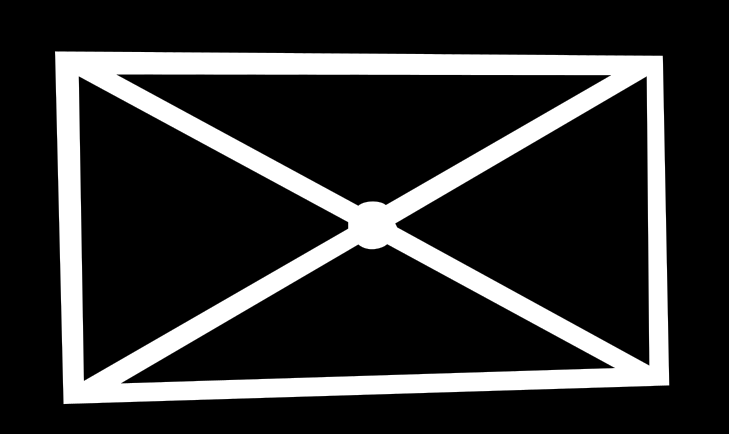
\includegraphics[scale=0.6]{img/mask.png}
\caption{Kleurenmasker van een scherm}
\end{figure}

Niet enkel de associatie van de gemaskeerde pixels wordt op deze manier behouden, maar deze methode maakt ook dat de komende bewerkingen maar over een minimale bounding box uitgevoerd worden ten opzichten van de volledige pixel matrix.
De afbeelding dat op elk slave-screen afgebeeld wordt voor detectie, is een combinatie van vorige iteraties van het project. Het combineren van een border met een kruis geeft het meeste informatie over de associatie van de kleur-gefilterde pixels bij overlap of afgedekte delen van het scherm en bovendien meer informatie over de oriëntatie van het scherm op de foto.

\subsection{Hoekpunten}
In de eerste stap wordt er bepaald of het scherm voornamelijk recht of gekanteld is ten opzichte van de foto. Hiervoor wordt langs de linker kant van het kader nagegaan hoe hoog de standaarddeviatie van witte pixels is. Bij een standaardafwijking onder de 15\% wordt een scherm als liggend of verticaal gezien op de foto.\\
Er werden vooraf algemene hoek-detectie algoritmes zoals shi-tomashi geïmplementeerd en getest, maar gaven een te complex resultaat op de binaire maskers om de juiste hoeken te filteren. Dit algoritme draagt ook een relatief grote overhead door de x- en y-sobel operaties die in een eerste stap toegepast moeten worden. Onze algoritmes zijn veel simplistischer, maar geven een perfect bruikbaar resultaat voor onze noden.\\
Als in eerste instantie het scherm als gedraaid beschouwd wordt, zal er vanuit elke rand van de bounding box van het eiland het de eerste mask-pixel als corner beschouwd worden. In het geval dat het scherm relatief horizontaal of verticaal recht staat, zal er loodrecht op de randen gezocht worden, maar volgens een diagonaal tot een mask-pixel [zie afbeeldingen].\\

\begin{figure}[h]
\centering
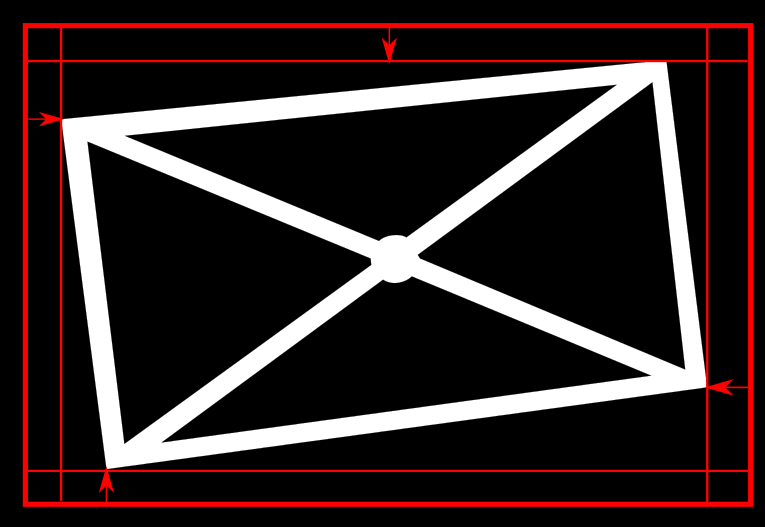
\includegraphics[scale=0.6]{img/perpSearch.png}
\caption{Loodrechte search}
\end{figure}

Beide variaties van hoek-detectie zal altijd vier hoeken als resultaat opleveren. Dit zullen door overlap en foutjes in het maskeren niet altijd correcte hoeken zijn. Na het bepalen, worden de hoeken nagekeken of deze resultaten wel degelijk kwalificeren als hoek. Deze kwalificatie is gebaseerd op bepaalde eigenschappen die in de buurt van elke hoek moeten gevonden worden, namelijk twee lijnen die tot de boord behoren en een diagonaallijn die naar het middelpunt van het scherm loopt \ref{fig:foute hoek}. Deze lijnen zijn bepaald door te filteren door de border- en diagonaal-kleur die gescheiden zijn door een witte rand (*beter verwijzen naar waar calccircle wordt uitgelegd in reconstructie?). Als in een eerder gevonden hoek deze voorwaarden niet aanwezig zijn, wordt deze hoek verworpen \ref{fig:correcte hoek}. \\

\begin{figure}[h] 
\centering
\begin{subfigure}{0.5\textwidth}
\label{fig:correcte hoek}
\centering
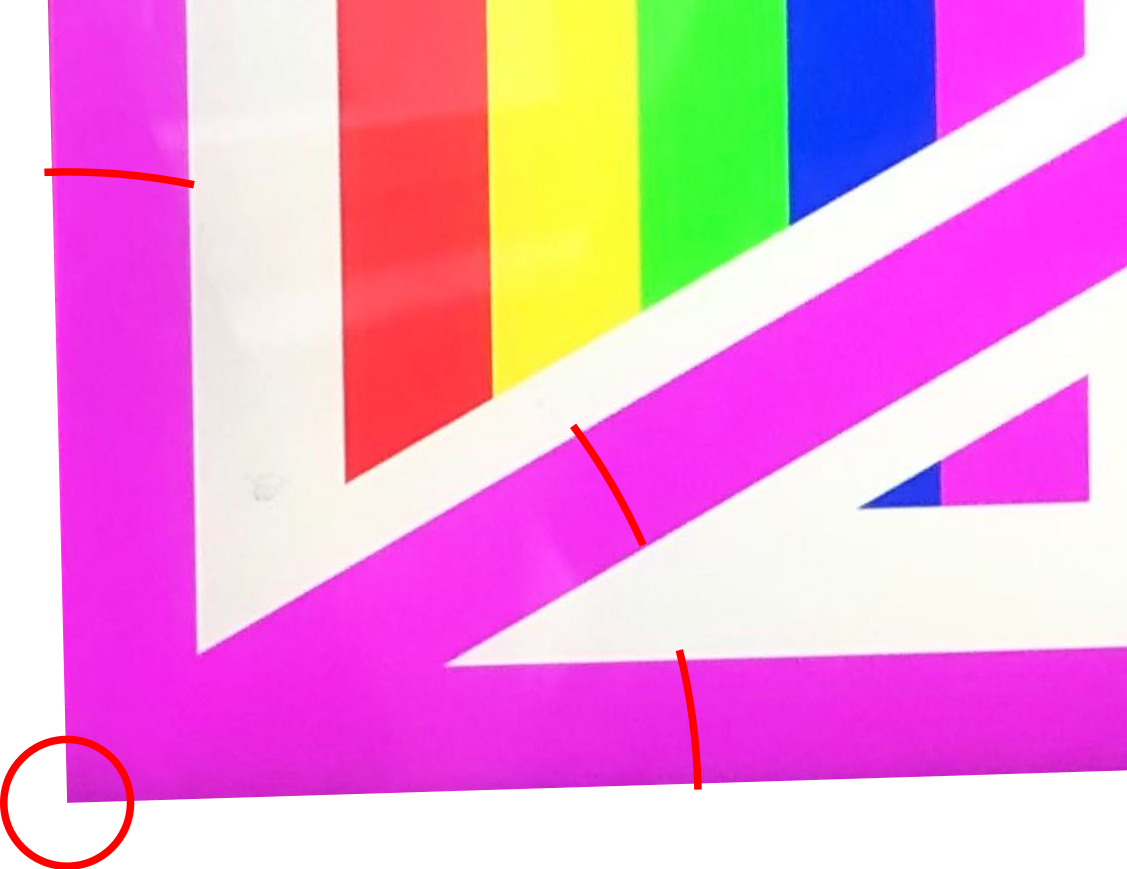
\includegraphics[width=0.6\textwidth]{img/correctCorner.png}
\caption{Een correcte hoek}
\end{subfigure}%
\begin{subfigure}{0.5\textwidth}
\label{fig:foute hoek}
\centering
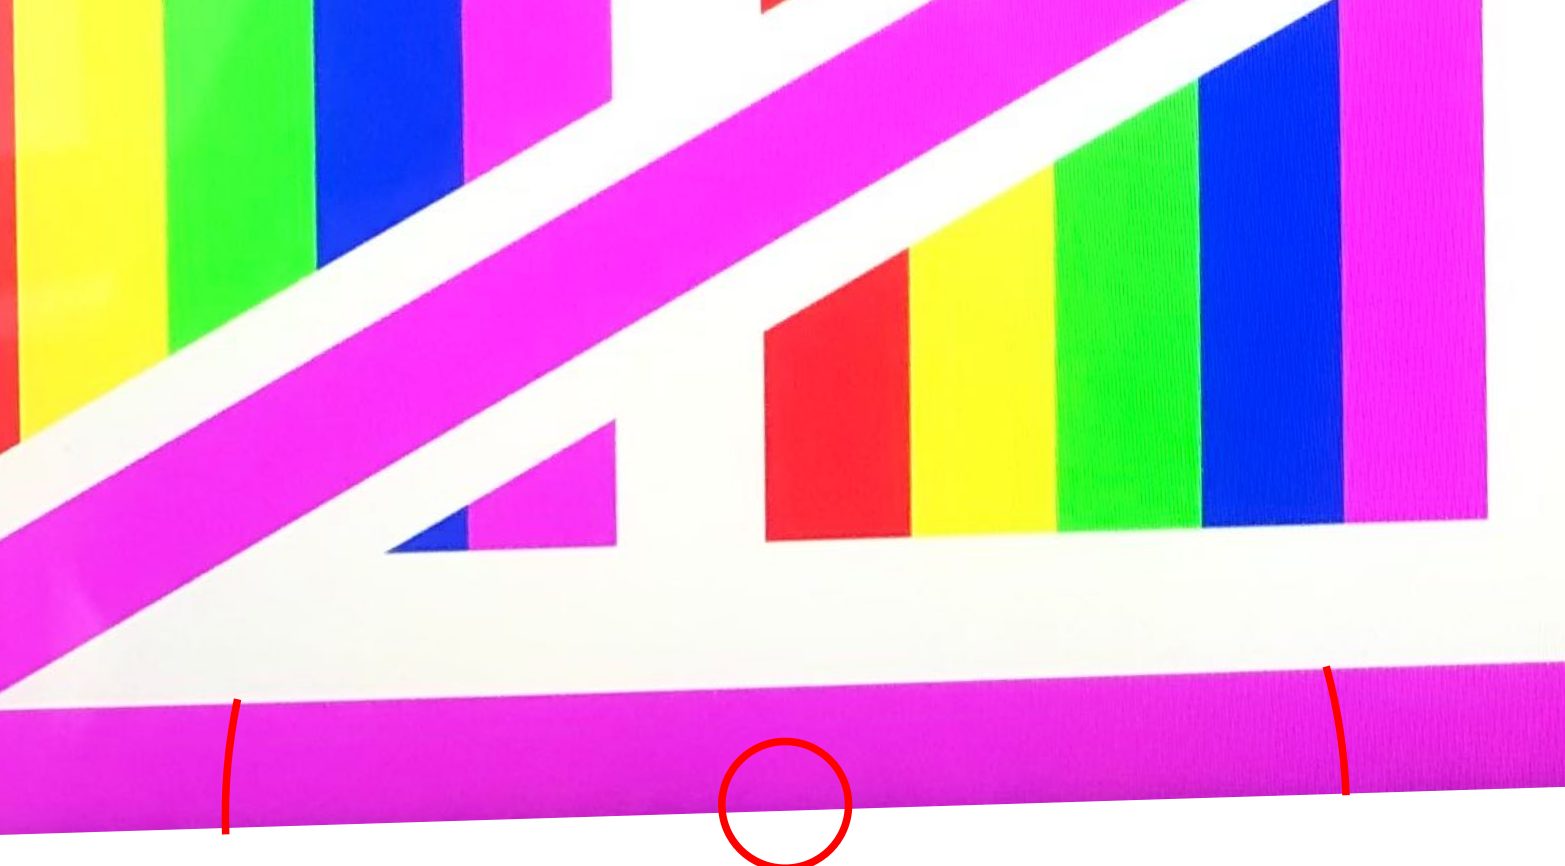
\includegraphics[width=0.6\textwidth]{img/notACorner.png}
\caption{Hoek zonder volledige features}
\end{subfigure}{}
\end{figure}

(linken/binden naar reconstruction) Als er geen vier correcte hoeken gevonden worden, zullen missende hoeken gereconstrueerd worden uit de wel gevonden hoeken en het middelpunt.